
\documentclass[a4paper, 10pt]{IEEEconf}  

\usepackage{geometry}
\geometry{a4paper, margin=1in}
  
  
\usepackage{subcaption}  
\usepackage[export]{adjustbox}    
\usepackage{verbatim}
\usepackage{graphicx}
\usepackage{pdfpages}
\usepackage{cite}
\usepackage{listings}
\usepackage{float}
\usepackage{url}
\usepackage{hyperref}
\usepackage{fancyhdr}
\usepackage{multicol}

\lstset{
	tabsize=2,
	breaklines=true
}

\setlength{\parskip}{1em}
\onecolumn

\title{\LARGE \bf Assignment 2: TensorFlow Neural Network Training\\Industrial Systems Design and Integration 282 772}
\author{Marc Alexander Sferrazza \\ 12164165
\thanks{This work was not supported by any organization}
\thanks{Faculty of Mechatronics Engineering, Massey University, Albany, Auckland, New Zealand
        {\tt\small Progress of project: https://github.com/alex1v1a/Industrial-Systems-Design-and-Integration} } }

\begin{document}

\maketitle
%\begin{figure}[h]
%\begin{subfigure}{0.5\textwidth}
%\includegraphics[width=1.5\textwidth, left]{images/ROS} 
%%\caption{ROS}
%\label{fig:ROS}
%\end{subfigure}
%\begin{subfigure}{0.5\textwidth}
%\includegraphics[width=0.3\textwidth, right]{images/gazebo}
%%\caption{Gazebo} 
%\label{fig:Gazebo}
%\end{subfigure}
%%\caption{Caption for this figure with two images}
%%\label{fig:image2}
%\end{figure}
\begin{figure}[H]
  \begin{center}
  
\includegraphics[width=110mm]{images/tf}
  \label{fig:kinetic}
  \end{center}
\end{figure}
\thispagestyle{empty}
\pagestyle{plain}


%%%%%%%%%%%%%%%%%%%%%%%%%%%%%%%%%%%%%%%%%%%%%%%%%%%%%%%%%%%%%%%%%%%%%%%%%%%%%%%%

\begin{abstract}
In this documentation TensorFlow's neural network machine learning is used to find a function for y=f(x) given some inputs and outputs. The process involves using the Multi-Layered Perceptron (MLP) technique training and placeholders are used to provide input.
\end{abstract}


\clearpage
\thispagestyle{empty}
\tableofcontents
\begingroup
\let\clearpage\relax
\listoffigures
%\listoftables
\endgroup
%\thispagestyle{empty}
\clearpage
\twocolumn

%%%%%%%%%%%%%%%%%%%%%%%%%%%%%%%%%%%%%%%%%%%%%%%%%%%%%%%%%%%%%%%%%%%%%%%%%%%%%%%%
%%%%%%%%%%%%%%%%%%%%%%%%%%%%%%%%%%%%%%%%%%%%%%%%%%%%%%%%%%%%%%%%%%%%%%%%%%%%%%%%
\clearpage
\setcounter{page}{1}
%\thispagestyle{empty}
\onecolumn

\section{INTRODUCTION}




%%%%%%%%%%%%%%%%%%%%%%%%%%%%%%%%%%%%%%%%%%%%%%%%%%%%%%%%%%%%%%%%%%%%%%%%%%%%%%%%

\subsection{Installation}

m is written to check the status of the install with success.

\begin{figure}[H]
  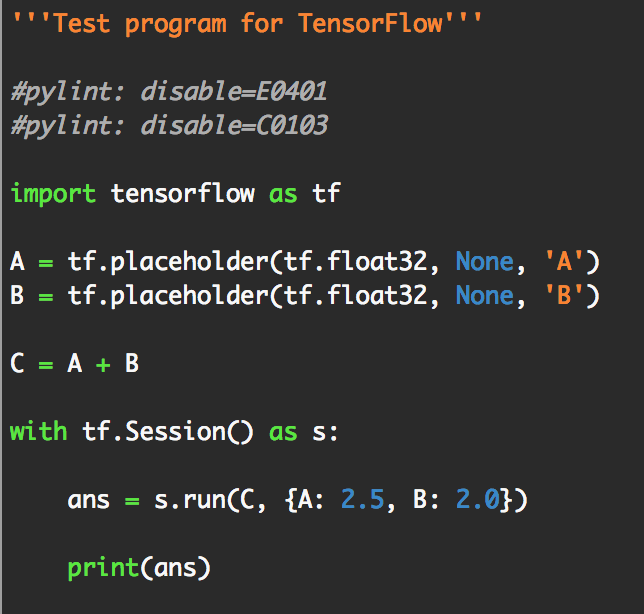
\includegraphics[width=0.5\linewidth, center]{images/test}
  \caption{Test file to check the working status for TensorFlow install, Result = 4.5}
  \label{fig:Test file to check the working status for TensorFlow install, Result = 4.5}
\end{figure}

%%%%%%%%%%%%%%%%%%%%%%%%%%%%%%%%%%%%%%%%%%%%%%%%%%%%%%%%%%%%%%%%%%%%%%%%%%%%%%%%
%%%%%%%%%%%%%%%%%%%%%%%%%%%%%%%%%%%%%%%%%%%%%%%%%%%%%%%%%%%%%%%%%%%%%%%%%%%%%%%%
%\clearpage
\section{METHOD}
 

%%%%%%%%%%%%%%%%%%%%%%%%%%%%%%%%%%%%%%%%%%%%%%%%%%%%%%%%%%%%%%%%%%%%%%%%%%%%%%%%

\subsection{Multi-Layered Perceptron (MLP) Training}

%%%%%%%%%%%%%%%%%%%%%%%%%%%%%%%%%%%%%%%%%%%%%%%%%%%%%%%%%%%%%%%%%%%%%%%%%%%%%%%%
%\clearpage
\subsection{Importing the CSV}

%%%%%%%%%%%%%%%%%%%%%%%%%%%%%%%%%%%%%%%%%%%%%%%%%%%%%%%%%%%%%%%%%%%%%%%%%%%%%%%%
%\clearpage
\subsection{Nodes}


%%%%%%%%%%%%%%%%%%%%%%%%%%%%%%%%%%%%%%%%%%%%%%%%%%%%%%%%%%%%%%%%%%%%%%%%%%%%%%%%
%\clearpage
\subsection{Base Optimizer}


%%%%%%%%%%%%%%%%%%%%%%%%%%%%%%%%%%%%%%%%%%%%%%%%%%%%%%%%%%%%%%%%%%%%%%%%%%%%%%%%
%%%%%%%%%%%%%%%%%%%%%%%%%%%%%%%%%%%%%%%%%%%%%%%%%%%%%%%%%%%%%%%%%%%%%%%%%%%%%%%%

\section{RESULTS}

Original Data set \& Inferred Output is shown 

An image illustrating the original data set and the inferred output of your program.

After successfully configuring the Multi-Layered Perceptron (MLP), reading in the values in the provided csv

\begin{figure}[H]
  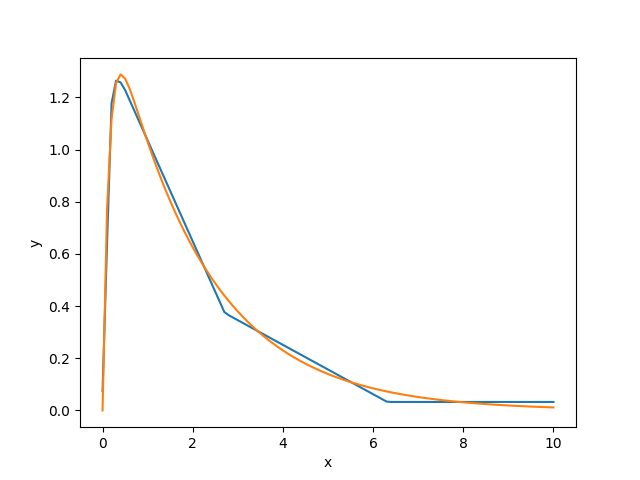
\includegraphics[width=0.8\linewidth, center]{images/plot}
  \caption{The final resultant is shown in compare on a graph}
  \label{fig:The final resultant is shown in compare on a graph}
\end{figure}

Once the initial results were found, to further the accuracy of the output the training of the MLP using the Adam Optimiser algorithum was used as suggested in class, please see variable for assigned learn rate in the code in the appendix. Below is the revised version using the Adam optimiser with specified nodes and learning rates as described in the logic documentation \cite{adam}. A clear difference between the optimiser reflects the accuracy for the learning of the function in this case.

\begin{figure}[H]
  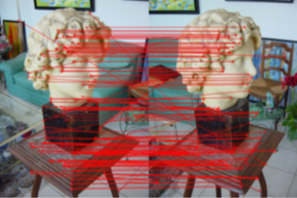
\includegraphics[width=0.8\linewidth, center]{images/3}
  \caption{The final resultant is shown in compare on a graph}
  \label{fig:The final resultant is shown in compare on a graph}
\end{figure}


%%%%%%%%%%%%%%%%%%%%%%%%%%%%%%%%%%%%%%%%%%%%%%%%%%%%%%%%%%%%%%%%%%%%%%%%%%%%%%%%
%%%%%%%%%%%%%%%%%%%%%%%%%%%%%%%%%%%%%%%%%%%%%%%%%%%%%%%%%%%%%%%%%%%%%%%%%%%%%%%%

\clearpage
\onecolumn
\section*{APPENDIX}
\begin{lstlisting}[language = Python]

\end{lstlisting}

\end{document}
